\documentclass[10pt,fleqn]{article}

\usepackage[english]{babel}
\usepackage[utf8x]{inputenc}
\usepackage{enumerate}
\usepackage{amsmath}
\usepackage{amssymb}
\usepackage{amsfonts} 
\usepackage{mathtools}
\usepackage{graphicx}
\usepackage{bm}
\usepackage[usenames,dvipsnames]{color}
\usepackage{todonotes}
\usepackage{dsfont}
\usepackage{hyperref}
\hypersetup{
    colorlinks,
    citecolor=black,
    filecolor=black,
    linkcolor=black,
    urlcolor=black
}
\usepackage{algorithm}
\usepackage{algorithmic}
\usepackage{appendix}
\usepackage{subcaption}
\usepackage{fancyvrb}
\usepackage{subfigure}
\usepackage{graphicx,xcolor}
\usepackage{pifont,mdframed}
\usepackage{tikz}
\usepackage{bm}
\usetikzlibrary{fit,positioning}


%
% Macros
%
\newcommand \cashort[1] { {\todo[color=yello]{#1 -- Cedric}} }
\newcommand \calong[1]  { { \todo[inline,color=yellow]{#1 -- Cedric} } }
\newcommand \gbshort[1] { {\todo[color=cyan!40]{#1 -- Guillaume}} }
\newcommand \gblong[1]  { { \todo[inline, color=cyan!40]{#1 -- Guillaume} } }
\newcommand \mgshort[1] { {\todo{#1 -- Mark}} }
\newcommand \mglong[1]  { { \todo[inline]{#1 -- Mark} } }
\newcommand \bfshort[1] { {\todo[color=green!40]{#1 -- Bryan}} }
\newcommand \bflong[1]  { { \todo[inline,color=green!40]{#1 -- Bryan} } }


% Adds a plus const to the end of a math expression
\def \pcst{+\text{const}}

% A fancy version for capital R
\def \Rcal{\mathcal{R}}

% A fancy version for r
\def \rcal{\mathbf{r}}

% Loss function / log likelihood as appropriate
\def \L{\mathcal{L}}

% KL divergence [Math Mode]
\newcommand{\kl}[2] {
	\text{KL}\left[#1||#2\right]
}

\newcommand \vecf[1] {
    \text{vec}\left(#1\right)
}

\newcommand \ent[1] {
    \text{H} \left[ #1 \right]
}

\newcommand \mut[2] {
    \text{I} \left[ #1 ; #2 \right]
}

\newcommand \dvi[2] {
    \text{D}_\text{VI} \left[ #1; #2 \right]
}

% Starts an expected value expresses [Math Mode]
\newcommand{\starte}[1] {%
	\mathbb{E}_{#1}\left[
}

% Ends an expected value expression [Math Mode]
\def \ende{\right]}

% Starts an varianc expresses [Math Mode]
\newcommand{\startv}[1] {%
	\mathbb{V}\text{ar}_{#1}\left[
}

% Ends an variance expression [Math Mode]
\def \endv{\right]}

%\newcommand \ex[2] {
%    \bigl\langle #1 \bigr\rangle_{#2}
%}
\newcommand \ex[2] {
    \mathbb{E}_{ { #2 } }\left[ #1 \right]
}
\newcommand \var[2] {
    \mathbb{V}ar_{ { #2 } }\left[ #1 \right]
}

\newcommand \halve[1] {
	\frac{#1}{2}
}

\newcommand \half {
    \halve{1}
}

\newcommand \tr { \text{tr} } 

\newcommand \T { ^\top } 

\newcommand \fixme[1] {
    {\color{red} FIXME: #1}
}

\newcommand \vv[1] { \bm #1 }

\newcommand{\mbeq}{\overset{!}{=}}

\newcommand \diag[1] { \text{diag} \left( {#1} \right) }
\newcommand \diagonal[1] { \text{diagonal} \left( {#1} \right) }

\newcommand \Ed {{ \vv{\xi}_d}}
\newcommand \Edj {{\xi_{dj}}}
\newcommand \Edk {{\xi_{dk}}}
\newcommand \AEdj {{\Lambda(\xi_{dj})}}
\newcommand \AEdk {{\Lambda(\xi_{dk})}}
\newcommand \AEd  {{ \bm{\Lambda}(\bm{\xi}_d) }}

\newcommand \Axi { { \Lambda_{\xi} } }
\newcommand \bxi { { \vv{b}_{\xi} } }
\newcommand \cxi { { c_{\xi} } }


\newcommand \wdoc      { { \vv{w}_d } }
\newcommand \wdt[0]  { { w_{dt} } }
\newcommand \wdn[0]  { { \vv{w}_{dn} } }
\newcommand \wdnt[0]  { { w_{dnt} } }
\newcommand \wdd[0]   { { \vv w_{d} } }
\newcommand \zd[0]   { { \vv z_{d} } }
\newcommand \zdn[0]  { { \vv{z}_{dn} } }
\newcommand \zdnk[0] { { z_{dnk} } }
\newcommand \zdk[0]  { { z_{dk} } }
\newcommand \thd[0]  { { \vv \theta_d } }
\newcommand \thdk[0] { { \theta_{dk} } }
\newcommand \thdj[0] { { \theta_{dj} } }
\newcommand \epow[1] { { e^{#1} } }
\newcommand \pkt     { { \phi_{kt}  } }
\newcommand \pk      { { \vv \phi_k } }
\newcommand \lmd     { { \vv \lambda_d } }
\newcommand \lmdk    { { \lambda_{dk} } }
\newcommand \xd      { { \vv x_d } }
\newcommand \atxd     { A ^\top \bm x_d}
\newcommand \axd     { A\bm x_d}
\newcommand \tsq      { { \tau^2 } }
\newcommand \ssq      { { \sigma^2 } }
\newcommand \tmsq     { { \tau^{-2} } }
\newcommand \asq      { { \alpha^2 } }
\newcommand \amsq     { { \alpha^{-2} } }
\newcommand \sgsq     { { \sigma^2 } }
\newcommand \xvec     { { \vv{x} } }
\newcommand \omk      { { \bm \omega _k } }
\newcommand \omkt     { { \omega_{kt} } }
\newcommand \oma     { { \Omega_A } }
\newcommand \gdn      { { \vv{\gamma}_{dn} } }
\newcommand \gdnk     { { \gamma_{dnk} } }
\newcommand \gdk      { { \gamma_{dk} } }
\newcommand \isigt   { { \Sigma^{-1}_{\bm \theta} } }




\newcommand \halfSig { \frac{1}{2\sigma^2} }

\newcommand \nor[2]   { \mathcal{N} \left( {#1}, {#2} \right) }
\newcommand \nord[3]   { \mathcal{N}_{#1} \left( {#2}, {#3} \right) }
\newcommand \mnor[3]  { \mathcal{N} \left(#1, #2, #3\right) }
\newcommand \norp[3]  { \mathcal{N} \left(#1; #2, #3\right) }
\newcommand \mnorp[4] { \mathcal{N} \left(#1; #2, #3, #4\right) }
\newcommand \mul[1]   { \mathcal{M} \left( {#1} \right) }
\newcommand \muln[2]  { \mathcal{M} \left( {#1},{#2} \right) }
\newcommand \dir[1]   { \mathcal{D} \left( {#1} \right) }
\newcommand \pois[1]  { \mathcal{P} \left( {#1} \right) }
\newcommand \gp[2]    { \mathcal{GP} \left( {#1}, #2 \right) }
\newcommand \dir[1]   { \mathcal{D} \left( {#1} \right) }
\newcommand \gam[2]   { \mathcal{G} \left( {#1}, {#2} \right) }
\newcommand \beta[1]  { \mathcal{B}eta \left( {#1}, {#2} \right) }

\newcommand \lne[1]  { { \ln \left( 1 + e^{ #1 } \right) } }
\newcommand \Tr[1]   { \tr \left(  {#1}  \right) }

\newcommand \roud  { \vv{\rho}_{d}  }
\newcommand \rodk { \rho_{dk} }

\newcommand \exA[1]  { \ex{#1}{q(A)} }
\newcommand \exV[1]  { \ex{#1}{q(V)} }
\newcommand \exT[1]  { \ex{#1}{q(\Theta)} }
\newcommand \extd[1] { \ex{#1}{q(\thd)} }
\newcommand \exTV[1] { \ex{#1}{q(\Theta)q(V)} }

\newcommand \Real[0]  { { \mathbb{R} } }
\newcommand \VReal[1] { { \mathbb{R}^{#1} } }
\newcommand \MReal[2] { { \mathbb{R}^{#1 \times #2} } }
\newcommand \Nat[0]  { { \mathbb{N} } }
\newcommand \VNat[1] { { \mathbb{N}^{#1} } }
\newcommand \MNat[2] { { \mathbb{N}^{#1 \times #2} } }

\newcommand \inv[1] { {#1}^{-1} }
\newcommand \invb[1] { \inv{\left( #1 \right)} }

\newcommand \cn { \textsuperscript{\texttt{[{\color{blue}Citation Needed}]}} }

\newcommand \const { { \text{c} } }

\providecommand \floor [1] { \left \lfloor #1 \right \rfloor }
\providecommand \ceil [1] { \left \lceil #1 \right \rceil }


\newcommand \vt[2] { { #1^{(#2)} } }

\newcommand \hashtag[1] { { \ttfamily \##1 } }

\newcommand \mvy  { \vv{m}_{\vv{y}} }
\newcommand \sigvy { { S_Y } }

\newcommand \mmy  { M_Y      }
\newcommand \md   { \vv{m}_d }
\newcommand \phin { \vv{\phi}_n }
\newcommand \isigma { { \inv{\Sigma} } }

\newcommand \sigv     { { \Sigma_V } }
\newcommand \isigv     { { \Sigma^{-1}_V } }

\newcommand \sigy { { \Sigma_Y } }
\newcommand \isigy { { \Sigma_{-1}_Y } }


\newcommand \omy  { { \Omega_Y } }
\newcommand \iomy { { \inv{\Omega_Y} } }

\newcommand \siga     { { \Sigma_A } }
\newcommand \isiga     { { \Sigma^{-1}_A } }
\newcommand \diagv { { \diag{\nu_1,\ldots,\nu_P} } }

\newcommand \ma { \vv{m}_a }
\newcommand \my { \vv{m}_y }

\newcommand \VoU { V \otimes U }

\newcommand \one { \mathbb{1} }
%\newcommand \one  {{  \mathds{1} }}

\newcommand \lse { \text{lse} }
%\newcommand \lse[0] { \mathrm{lse} }

% Conditional independence 
\def\ci{\perp\!\!\!\perp} % from Wikipedia



% ------ For the eval section

% Multinomial PDF [Math Mode]
% params: 1 - the variable
%         2 - the value
%         3 - the state indicator (e.g. k for a distro with K values)
%         4 - any additional subscript
\newcommand{\mpdf}[4] {
	\prod_{#3} {#1}_{{#4} {#3}} ^ {#2}
}

% Dirichlet PDF [Math Mode]
% params: 1 - the variable
%         2 - the hyper-parameter
%         3 - the state indicator (e.g. k for a distro with K values)
%         4 - any additional subscript
\newcommand{\dpdf}[4] {
	\frac{1}{B({#2})} \prod_{#3} {#1}_{{#4} {#3}} ^ {({#2}_{#3} - 1)}
}

% To simplify the sampling equations, this is indicates
% that the given value has had datapoint "m" stripped out
%
\newcommand{\lm}[1] {
	#1^{\setminus m}
}

\newcommand \model[0] {
    \mathcal{M}
}

\newcommand \perplexity[1] {
    \mathcal{P} \left( { #1 } \right)
}

\newcommand \WTrain {
    \mathcal{W}^{(t)}
}

\newcommand \WQuery {
    \mathcal{W}^{(q)}
}

\newcommand \oneover[1] {
    \frac{1}{ {#1} }
}

\newcommand \samp[1] {
    { #1 }^{(s)}
}

\newcommand \etd[0] {
    \vv{\eta}_d
}

\begin{document}




\subsubsection{Evaluation Metrics}
\label{sec:eval}

A number of methods have been proposed to evaluate admixture models. By far the most popular is perplexity, which is defined as the geometric mean of the reciprocals of token likelihoods. The perplexity for a model $\model$ is defined as

\begin{align}
\perplexity{\model} = \sqrt[n_{d}]{\prod_d \prod_n \frac{1}{p(w_{dn}|\model)}} = \exp \left( \frac{-\sum_d \sum_n \ln p(w_{dn}|\model)}{n_{d\cdot\cdot}} \right) \label{eqn:perp_def}
\end{align}

To get some intuition about perplexity, a example cited by \cite{Goodman2001} is that a model that assigned equal probability to 100 words would be 100. The true distribution would be significantly \emph{lower} than this, and so lower perplexity scores are always preferable. This preference can be motivated from information theory, as taking the log of a perplexity score gives the entropy of the word likelihoods, and Shannon's theorem states that the entropy is the average number of bits (assuming one takes the log-base-two) required to encode each word using an ideal coding scheme.

Taking this further, perplexity can be shown to be a special case of the cross-entropy function $\text{H}[p,q]$ where $p(w_{dv})$ is the empirical distribution of the word, $q(w_{dv})$ is the distribution we've inferred (confusingly denoted $p(w_{dn})$ in \eqref{eqn:perp_def}), and we use $e$ as the base and the natural log in the exponent. 

To evaluate perplexity, one needs to determine the probability of a test, or query, set $\WQuery$ given the training set $\WTrain$. To simplify the notation, and make it clear which are the learnt parameters, we assume an LDA model in which the document-level topic distributions $\thd$ have been marginalised out, leaving a Polya distribution over the latent per-token topic-assignments $\zdn$, parameterised by a prior $\vv{\alpha}$.

\begin{align}
p(\WQuery|\WTrain) = \int p(\WQuery|\Phi, \vv{\alpha})p(\Phi,\vv{\alpha} | \WTrain) d\Phi d\vv{\alpha}
\end{align}

where due to the assumed exchangeability of documents $p(\WQuery|\Phi, \vv{\alpha}) = \prod_ p(\vv{w}_d|\Phi, \vv{\alpha})$. Leaving aside the first term in the integrand, one can approximate this integral either by substituting in point estimates for $\Phi$ and $\vv{\alpha}$ or sampling from the posterior - the latter being particularly easy in cases where the model parameters have been fit using Gibbs sampling.

The issue that remains however is how to evaluate $p(\vv{w}_d|\Phi, \vv{\alpha})$, which is dependant on the latent variables $\zdnk$. There are a number of ways in which this can be evaluated, of which two have been used frequently in the literature.

The harmonic mean method has been used in\cite{Griffiths2004}\cite{Griffiths2005}\cite{Wallach2006}, all of which performed inference using collapsed Gibbs samplers. The approach is defined as
\begin{align}
\oneover{p(w)} = \sum_z \frac{p(z|w)}{p(w|z)} \approx \oneover{S} \sum_s \oneover{p(w|\samp{z})}
\end{align}
where the approximation comes from implementing an importance sampler using the target $p(z|w)$ as the proposal distribution. Implementing this we can see that 

\begin{align}
p(\vv{w} | \Phi, \vv{\alpha}) \approx \text{HM}\left[ \left\{ p(\vv{w}|\samp{\vv{z}}, \Phi \right\}_{s=1}^{S}  \right]
\end{align}

where $\text{HM}\left[\cdot\right]$ is the harmonic mean, and the sampling distribution over $\zdnk$ is given by

\begin{align}
p(z_{dn} = k | \vv{w}_d, \vv{z}_d^{\setminus n}, \Phi, \vv{\alpha}) \propto \phi_{k,{w_{dn}}}\frac{n_{dk\cdot} + \alpha_k}{n_{d\cdot\cdot} + \sum_j \alpha_j}
\end{align}

The second approach is the left-to-right method, which has been used in \cite{Mimno2011} and \cite{Mimno2012a}. By factorising the likelihood as

\begin{align}
p(\vv{w}|\Phi, \vv{\alpha}) & = \prod_n p(w_n | \vv{w}_{<n}, \Phi, \vv{\alpha}) \\
& = \prod_n \sum_{\vv{z}_{<n}} p(w_n, \vv{z}_{<n}| \vv{w}_{<n}, \Phi, \vv{\alpha})
\end{align}
it is possible to approximate the likelihood using a variant a sequential Monte-Carlo, where each particle $p$ iteratively draws samples of $z^{(p)}_{dn'}$ for $n' \in 1 \ldots n_{d\cdot\cdot}$, and uses these samples to evaluate the overall probability of the likelihood. The full algorithm given in \cite{Wallach2009}.

When the harmonic mean, left-to-right and several other methods including importance sampling and annealed importance sampling where compared in \cite{Wallach2009} it was found that the harmonic mean method tended to ``wildly overestimate" the true likelihood, while the left-to-right method gave the most accurate estimate.

Another method by which perplexity can be evaluated is ``document-completion" which has been used in \cite{Virtanen2012a}\cite{Asuncion2012}\cite{RosenZvi2004}. Each document in the test-set is partitioned into two halves\footnote{Given that words are assumed exchangeable within documents, and that long documents may exhibit structure affecting which topics can be inferred where, one can, and indeed should, permute the word order before splitting each document}: an estimation fragment, $\vv{w}_d^{(e)}$, from which a topic distribution is inferred; and an evaluation document, $\vv{w}_d^{(l)}$, whose likelihood given the inferred topic distribution is calculated. Formally writing this as
\begin{align}
p(\vv{w}_d^{(l)}|\vv{w}_d^{(e)}, \Phi, \vv{\alpha}) = \frac{p(\vv{w}_d^{(l)},\vv{w}_d^{(e)} |\Phi, \vv{\alpha})}{p(\vv{w}_d^{(e)}|, \Phi, \vv{\alpha})}
\end{align}

it should be clear that the methods used above can be used to infer both $p(\vv{w}_d^{(e)}|, \Phi, \vv{\alpha})$ and $p(\vv{w}_d^{(l)},\vv{w}_d^{(e)} | \Phi, \vv{\alpha}) = p(\vv{w}_d | \Phi, \vv{\alpha})$. However the most  popular method used in this case is topic-estimation which involves sampling $\vv{z}_d^{(e,s)} \sim p(\vv{z}_n^{(e)} | \vv{w}^{(e)}, \Phi, \vv{\alpha})$ and then evaluating $\vv{\theta}_d^{(e)}$ as

\begin{align}
\theta^{(e)}_{dk} = p(k | \vv{z}^{(e,s)}, \vv{\alpha}) = \frac{n^{(e)}_{dk\cdot} + \alpha_k}{n^{(e)}_{d\cdot\cdot} + \sum_j \alpha_j}
\end{align}

from which one can then evaluate the probability of the evaluation document:

\begin{align}
p(\vv{w}_d^{(l)}|\vv{w}_d^{(e)}, \Phi, \vv{\alpha}) \approx
\oneover{S} \sum_s \prod_n \sum_k \phi_{k,w^{(l)}_{dn}}\theta_{dk}^{(e)}
\end{align}

In practice, particularly with variational approaches, a single point estimate of $\vv{\theta}_d^{(e)}$ may be used instead\cite{Asuncion2012}, though when evaluating document completion \cite{Wallach2009} found that the topic-estimation method, even when implemented via sampling, compared ``poorly" with left-to-right sampling. 

As we have shown, measures of perplexity are highly dependant on how the held-out likelihood was evaluated, something which is rarely described in the literature. A further issue, mentioned in \cite{Asuncion2012} is that the performance of topics models is highly sensitive to the configuration of hyper-parameters, something confirmed by their results and those of \cite{Wallach2006}. Thus care needs to be exercised when comparing measures of perplexity across different publications.

A further argument against perplexity was made by \cite{Chang2009} which asked human testers to inspect the topic vocabularies generated by different topic models (LDA, CTM and PLSA). Tests included ``word-intrusion" experiments, where in a list of topic-words testers had to detect a ``wrong" word added by the experiments from a different topic, and ``topic-intrustion", where in a list of documents excerpts belonging to a single topic, testers had to detect a ``wrong" document added by the experiments from a different topic. The CTM model, despite achieving the best perplexity score, faired worst in both of these tasks. Additionally, in \cite{Azzopardi2003} it was shown that when using language-models to aid information retrieval, language models with the best perplexity scores did not always lead to the best precision scores. In light of this, some more recent publications such as \cite{Li2006}\cite{Wang2007}\cite{Lindsey2012} have used similar intrusion tests via Mechanical Turk to test the performance of their models.

Between these two extremes, other metrics exist, however. The ``topical coherence" metric was first introduced in \cite{Mimno2011} and additionally used in \cite{Mimno2012a} directly addresses the word-intrusion problem. One can assume that if a set of words all belong to a single topic, one would see most of them occur in a single document belonging to that topic, and not see occur uniformly across all documents and all topics. Therefore letting $D(t)$ be the number of documents where word $t$ occurs at least once, and $D(t,v)$ be the number of documents containing at least once occurrence each of both $t$ and $v$, the coherence metric is defined as
\begin{align}
C(t,V^{(k)}) = \sum_{m=2}^{M} \sum_{l=1}^{m-1} \ln \frac{D(v_{km}, v{kl}) + 1}{D(v_{kl})}
\end{align}
where $V_k$ is the set of the $M$ most probable words in topic $k$, and the addition of $1$ to the numerator is to avoid taking the log of zero. 

%\fixme{Read this some more. Also pointwise mutual info}

The \emph{empirical likelihood} of \cite{Li2006} tests the generative ability of a model. For each test document, this involves using the model to generate, say, 1,000 synthetic documents, deriving an empirical (in this case multinomial) distribution from each document, and then evaluating the average of the probabilities of the test document according to each of these empirical distributions. This has additionally been used in \cite{Doyle2009}\cite{Mimno2008}. In \cite{Wallach2009} it was shown that this method is an approximation to $p(\vv{w}_d|\Phi, \vv{\alpha}) = \int p(\vv{w}_d, \thd | Phi)p(\thd|\vv{\alpha})d\thd$ using importance sampling with true posterior employed as a proposal distribution. Were the synthetic documents infinitely long, the two methods would be identical. This analogy points to a potential deficiency of this method however, which is that one would expect the variance of an estimate derived from importance sampling to be very high when sampling from high-dimensional distributions: consequently for very high topic-counts (500-topic cases are common) this may not be a reliable estimator.

\subsubsection*{Evaluation Against Labelled Data}
The problem of evaluation against labelled data indicates that there are two possible labelings, a 1-of-$K$ labelling $\vv{z}_d$ and a 1-of-$L$ labelling $\vv{t}_d$ say. When evaluating a clustering of a dataset against its labelling, many metrics exist. Of these the most well known is likely the F1-Score which is is the harmonic mean of precision, $p$ and recall, $r$, $F_1 = 2 \frac{p \cdot r}{p + r}$ where precision is $p=\frac{TP}{TP+FP}$ and $r=\frac{TP}{TP+FN}$ and $TP, FP, TN, FN$ refer to the true and false positives and negatives respectively.

In the presence of soft-clustering and multiple labels one can\footnote{See https://facwiki.cs.byu.edu/nlp/images/2/25/ClusterEvaluation.ppt} define an $F_1$ score for a single topic $k$ and a single label $l$ thusly.

Letting \emph{precision} be the ``number of documents in a cluster that belong there", and recall be be ``did all the documents that should be in this cluster make it in" we derive the following:
\begin{align}
p_{kl} & = \frac{n_{kl}}{n_k} = \frac{\sum_d \theta_{dk} t_{dl}}{\sum_d \theta_{dk}}  & r_{kl} & = \frac{n_{kl}}{n_l} = \frac{\sum_d \theta_{dk} t_{dl}}{\sum_d t_{dl}} \label{eqn:myrecall}
\end{align}

where $n_{kl}$ is the number of documents in cluster $k$ which have the label $l$ and $n_k$ is the number of documents in cluster $k$. We can, for a single topic $k$ and a single label $l$ specify the $F_1$ score as

\begin{equation}
F_1^{(k,l)} = 2 \frac{p_{kl} \cdot {r_{kl}}}{p_{kl} + {r_{kl}}}
\end{equation}

For a single label $l$ one can take the max across topics $F_1^{(l)} = \max_{k \in 1\ldots K} F_1^{(k,l)}$ and then finally describe the entire corpus using a weighted average of label specific $F_1$ scores, with the weights proportional to the number of documents with each label.

\begin{equation}
F_1 = \sum_l \frac{n_l}{D'} F_1^{(l)}
\end{equation}

where $D' = \sum_d \sum_l t_{dl}$ is the total number of label instances, to account for the fact that there may be documents with more than one label, and so $D' \geq D$.


\begin{figure}
  \centering
    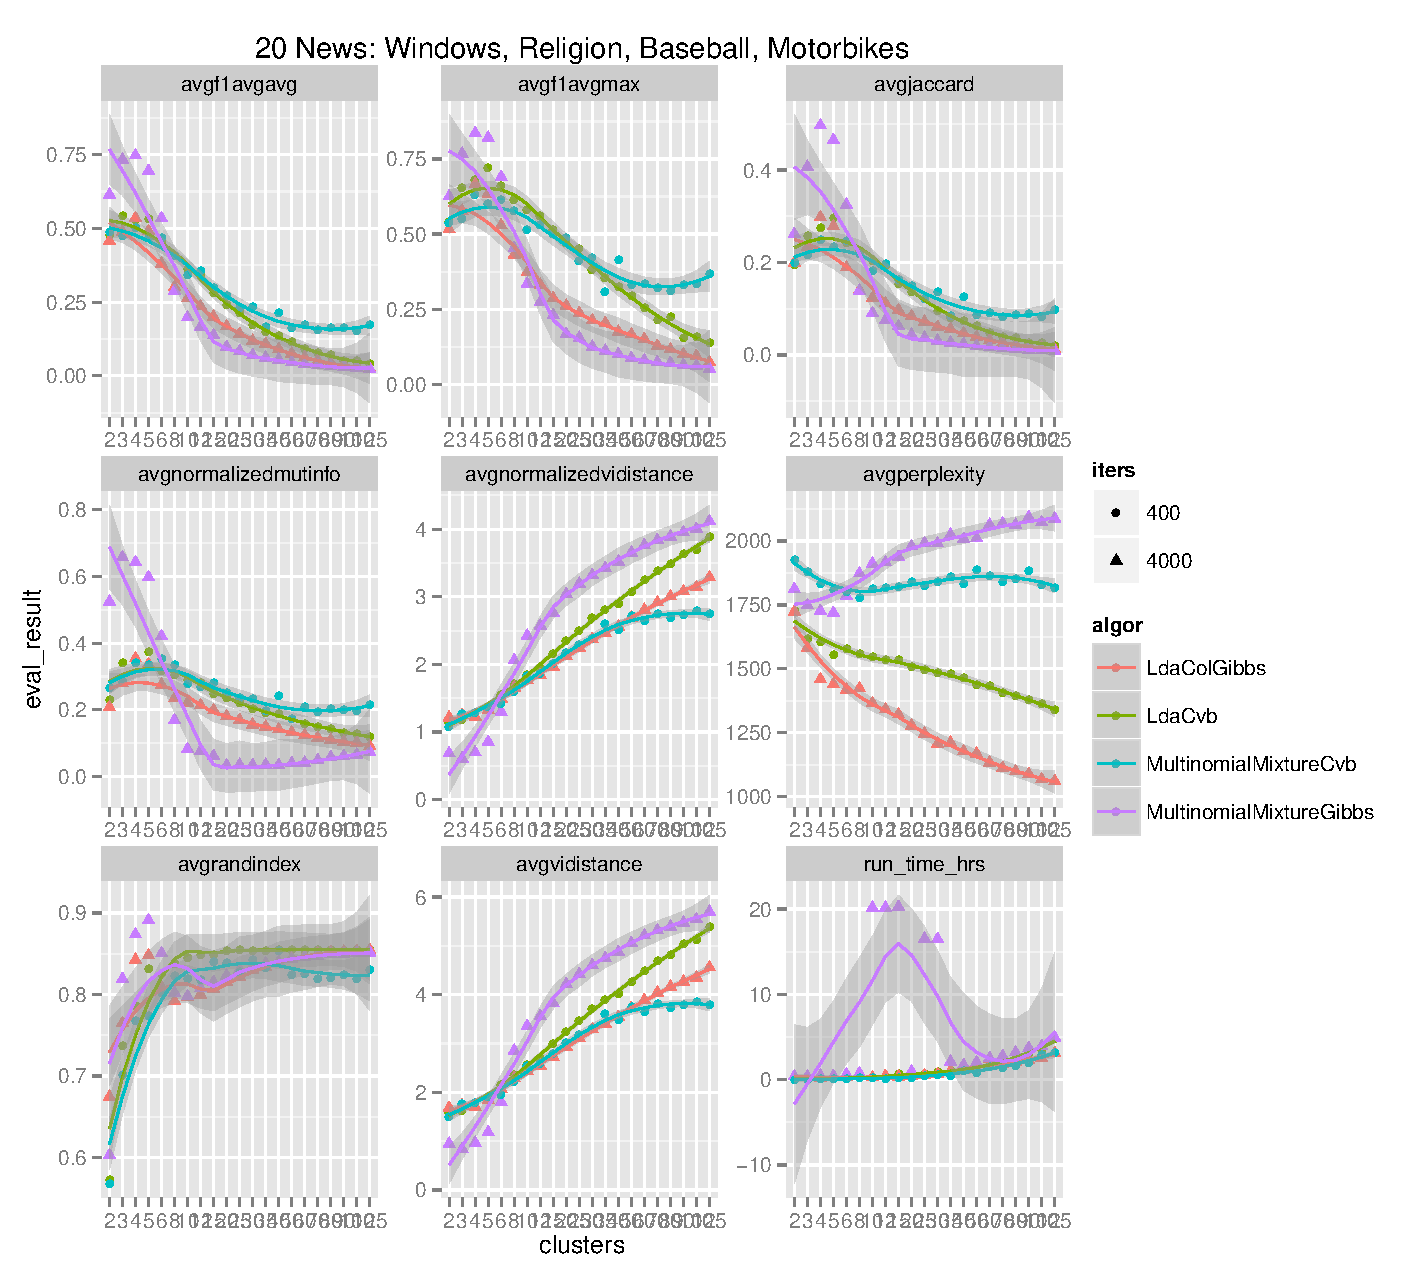
\includegraphics[width=0.9\textwidth]{plots/20news-2013-03-25.pdf}
  \caption{Results using different accuracy metrics for a mixture of multinomials and LDA on a subset of the 20-news dataset. Trendlines and shading are from a LOESS fit to the points. A variation of the soft F1 measure described in the text is shown where we average over label-specific F1 scores instead of taking the maximum. Held-out likelihood was evaluating using the document-completion metric with inferred topics.}
  \label{fig:eval-metrics-shootout}
\end{figure}


A different approach to comes from the intuition that given two equivalent labellings, one would expect label pairs $z=k$ and $t=l$ to co-occur, and so expect that $p(z,t) \neq p(z)p(t)$, which opens the door to a number of information theoretic measures such as normalised mutual information (NMI) and the Variation of Information (VI) distance..

\newcommand{\TopDist}{\Theta}
\newcommand{\LabDist}{\mathbb{C}}
\newcommand{\NMI}{\text{NMI}}

Given a corpus-wide distribution over topics $\TopDist$ and a corpus wide distribution over labels $\LabDist$ the NMI is defined as:

\begin{equation}
\NMI = \frac{\mut{\TopDist}{\LabDist}}{1/2(\ent{\TopDist} + \ent{\LabDist})}
\end{equation}

where the mutual information is defined as

\begin{equation}
\mut{\TopDist}{\LabDist} = \sum_k \sum_l p(\theta_{\cdot k}, t_{\cdot l}) \ln \frac{p(\theta_{\cdot k}, t_{\cdot l})}{p(\theta_{\cdot k})p(t_{\cdot l})}
\end{equation}

and the entropies are defined as

\begin{align}
\ent{\TopDist} & = - \sum_k p(\theta_{\cdot k}) \ln (\theta_{\cdot k}) &
\ent{\LabDist} & = - \sum_l p(t_{\cdot l}) \ln p(t_{\cdot l})
\end{align}

In the case of LDA these distributions would be defined as
\begin{align}
p(\theta_{\cdot k}) & =  \frac{1}{D} \sum_d \theta_{dk} ,&
p(t_{\cdot l}) &= \frac{1}{D'} \sum_d t_{dl} ,& 
p(\theta_{\cdot k}, t_{\cdot l}) & = \frac{1}{D'} \sum_d \theta_{dk} t_{dl}
\end{align}
where again $D' = \sum_d \sum_l t_{dl}$ is the total number of label instances, such that $D' \geq D$


The VI distance\cite{Meila2003} is another information-theoretic measure defined over a topic distribution $\TopDist$ and labelling distribution $\LabDist$ as:

\begin{equation}
\dvi{\TopDist}{\LabDist} = \ent{\LabDist} + \ent{\TopDist} - 2 \mut{\LabDist}{\TopDist}.
\end{equation}

$\dvi{\TopDist}{\LabDist}$ is a true metric: it is always non-negative, becomes zero if and only if $\LabDist = \TopDist$, is symmetric, and observes the triangle inequality, $\dvi{X}{Z} + \dvi{Z}{Y} \geq \dvi{X}{Y}$. However the range over which VI distance scores will take is dataset-dependant, and so to compare scores across datasets one can use the \emph{normalized VI distance}\cite{Reichart2009} which is defined as. 

\begin{align}
\text{NVI}\left[ \TopDist, \LabDist \right] = \left\{ \begin{array}{lr}
     \frac{1}{\ent{\TopDist}}\dvi{\TopDist}{\LabDist} & \ent{\TopDist} \neq 0 \\
     \ent{\LabDist} & \text{otherwise}
 \end{array}\right.
\end{align}


The VI distance has been used to compare topics inferred by LDA with manual labelling of over 20,000 news-stores in \cite{HeinrichEtAl2005}. 


A well-known metric from the field of clustering is the rand Rand Index, which determines how similar are two ways of partitioning data. It defines four counts
\begin{enumerate}[a.]
    \item The number of document-pairs which are in the same cluster and have the same label
    \item The number of document-pairs which are in different clusters but share the same label
    \item The number of document-pairs which are the the same cluster but have different labels
    \item The number of document pairs which are not in the same cluster and have different labels.
\end{enumerate}

Given these definitions the index is then $\text{RI} = \frac{a + d}{a + b + c + d}$. This is broadly similar to the idea of accuracy traditionally defined as being $\frac{TP + TN}{TP + FN + FP + TN}$

For the kind of soft-clustering featured in LDA, one would define these counts as
\begin{align}
a & = \sum_k \sum_{d, {p>d}} \theta_{dk} \theta_{pk} \sum_l t_{dl}t_{pl} & \quad
b & = \sum_k \sum_{d, {p>d}} \theta_{dk} (1 -\theta_{pk}) \sum_l t_{dl}t_{pl}\\
c & = \sum_k \sum_{d, {p>d}} \theta_{dk} \theta_{pk} \sum_{l,m \neq l} t_{dl}t_{ml} & \quad
d & = \sum_k \sum_{d, {p>d}} \theta_{dk} (1- \theta_{pk}) \sum_{l,m \neq l} t_{dl}t_{ml}
\end{align}

Plots of all these metrics, for different topic counts, are given in figure \ref{fig:eval-metrics-shootout} for documents taken from four very different newsgroups from the overall 20-newsgroups dataset.


\bibliographystyle{plain}
\bibliography{/Users/bryanfeeney/Documents/library.bib}

\end{document}


